\chapter{\glsdesc{MMLT}}

This chapter introduces the \gls{MMLT} problem and
some of its properties. First of all, the formal definition
of the problem:

\begin{problem}[\gls{MMLT}]
  \hfill
  \begin{labeling}{\hspace{4em}}
    \item[\textbf{Given:}]
      Set of points in the plane \(P\) and implicitly their induced segments
      \(S_P\) (see \cref{sec:pre_induced_segments})
    \item[\textbf{Sought:}]
      Triangulation \(\gls{Topt}\subseteq S_P\) of \(P\) which maximizes
      \(\min\limits_{s\in \gls{Topt}} |s|\) 
      with \(|s|\) being the length of the segment \(s\)
  \end{labeling}
\end{problem}

Note that an optimal solution for \gls{MMLT} need not be unique as
\cref{fig:non_unique_optimal} shows. As mentioned earlier, the
\gls{MMLT} problem is NP-complete \cite{mmlt_complexity}.

\begin{figure}[ht]
  \centering
  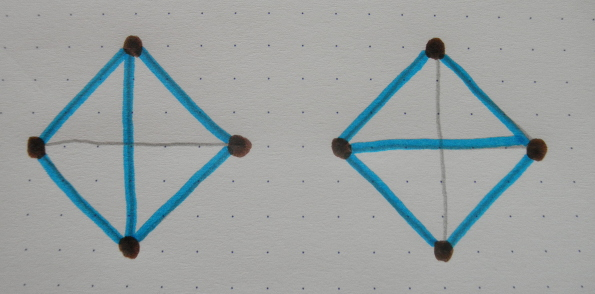
\includegraphics[width=0.5\textwidth]{img/non_unique_optimal.jpg}
  \todo[inline]{replace}
  \caption{Example of different optimal solutions for the same point set.\label{fig:non_unique_optimal}}
\end{figure}




\section{Intersection Graph}\label{sec:pre_intersection_graph}
For a point set \(P\) with \(n\) points in the plane 
the induced segments (see
\cref{sec:pre_induced_segments}) have \(\Theta(n^4)\) intersections.
\cite{quadrilaterals_bound} Thus calculating the intersection graph
takes \(\Omega(n^4)\) time.

\section{Separators}\label{sec:pre_separators}
The set of separators \(\gls{Ssep}[(s)]\) for a line segment
\(s\) are all induced line segments \(S_P\) that improve the
\gls{MMLT} solution, i.e. all with \(s\) \gls{cross} line segments
which are longer than \(s\):

\[
	\gls{Ssep}[(s)] := \{
		\gls{ssep} : \gls{ssep}\in S_P,
		|s| < |\gls{ssep}|\land~ s,\gls{ssep}~\gls{cross}
	\}
\]

\section{Short Segments}\label{sec:pre_short_segments}
Short segments are all segments shorter than a specific length:

\[
  \gls{Sshort}[(l)] := \{ s : \gls{ssep}\in S_P,~ |s| < l \}
\]



\section{Upper Bounds}
Every triangulation \(T\subseteq S_P\) of a point set \(P\) itself is
a maximum set of non-crossing segments. Therefore every segment 
\(s \in S_P\) that is not crossed by a segment \(s_c \in T\) has
to be part of \(T\). This leads to the following statement:

\begin{theorem}[upper bound]\label{thm:upper_bound}
  Given a point set \(P\) and its induced segments \(S_P\). Let
  \gls{Topt} be an optimal \gls{MMLT} solution for \(P\). Every
  segment \(s\) without separators is an upper bound for \gls{Topt}:
  \[
    \forall s \in S_P,~ \gls{Ssep}[(s)] = \emptyset :
    \min\limits_{s_{\min} \in \gls{Topt}} |s_{\min}| \leq |s|
  \]
  which is equivalent to
  \[
    \forall s \in S_P:~ \lnot\exists \gls{ssep} \in S_P :
    |s| < |\gls{ssep}| \land~ s, \gls{ssep}~ \gls{cross}
    \implies \min\limits_{s_{\min} \in \gls{Topt}} |s_{\min}| \leq |s|
  \]
\end{theorem}

\begin{proof}
  Assume \(
    \exists s \in S_P,~ \gls{Ssep}[(s)] = \emptyset :
    \min\limits_{s_{\min} \in \gls{Topt}} |s_{\min}| > |s|
  \). This implies \(s \not\in \gls{Topt}\) and
  \(\forall s' \in S_P,~ |s'| \leq |s| : s' \not\in \gls{Topt}\).
  Therefore \(\forall s_c \in S_P,~
   s, s_c~\gls{cross} : s_c \not\in \gls{Topt}\). This means 
   that for \gls{Topt} to be a triangulation \(s\) has to be in
   \gls{Topt} -- which is a contradiction.
\end{proof}

This upper bound is not tight as can be seen in
\cref{fig:upper_bound_tightness}. One of the short segments (red)
has to be in an optimal \gls{MMLT} solution because their separators
(green) cross. The short segments are clearly shorter than the 
segments without separators (blue).

\begin{figure}[ht]
  \centering
  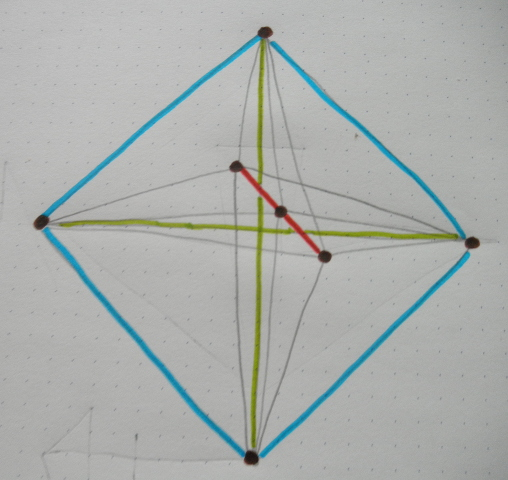
\includegraphics[width=0.5\textwidth]{img/upper_bound_tightness.jpg}
  \todo[inline]{replace}
  \caption{\label{fig:upper_bound_tightness}Example where the upper
    bound from \cref{thm:upper_bound} is not tight.}
\end{figure}

\begin{definition}[shortest non-separable segment]
  For a set of points in the plane \(P\) and its induced segments
  \(S_P\) let the shortest non-separable segment \gls{snose} be:
  \[ \gls{snose} := \argmin\limits_{s \in S_P,~\gls{Ssep}[(s)] = \emptyset} |s| \]
\end{definition}

\Cref{thm:upper_bound} can be generalized by taking
conflicting separators into account. A segment may be part of an
optimal \gls{MMLT} solution because all of its separators interfere
with those of a shorter segment.

\begin{theorem}[tight upper bound]\label{thm:tight_upper_bound}
  Given a point set \(P\) and its induced segments \(S_P\). Let
  \gls{Topt} be an optimal \gls{MMLT} solution for \(P\). Let
  \(S_\textnormal{conf}(s)\) be the potentially conflicting
  separators for a segment \(s\):
  \[
    \gls{Sconf}[(s)] :=
      \gls{Topt} \cap \bigcup_{s' \in \gls{Sshort}[(|s|)]}
      \gls{Ssep}[(s')]
  \]
  Every segment \(s\) without non-conflicting separators is an upper
  bound for \gls{Topt}:
  \[
    \forall s \in S_P,~ 
    \{
      \gls{ssep} \in \gls{Ssep}[(s)] : 
      \gls{ssep} \cup \gls{Sconf}[(s)]~\gls{ncross}
    \} = \emptyset :
    \min\limits_{s_{\min} \in \gls{Topt}} |s_{\min}| \leq |s|
  \]
\end{theorem}

\begin{proof}
  This proof is very similar to the proof of \cref{thm:upper_bound}.
  Assume
  \[
    \exists s \in S_P,~ 
    \{
      \gls{ssep} \in \gls{Ssep}[(s)] : 
      \gls{ssep} \cup \gls{Sconf}[(s)]~\gls{ncross}
    \} = \emptyset :
    \min\limits_{s_{\min} \in \gls{Topt}} |s_{\min}| > |s|
  \]
  which implies \(s \not\in \gls{Topt}\) and
  \(\forall s' \in S_P,~ |s'| \leq |s| : s' \not\in \gls{Topt}\).
  
  If \(\gls{Ssep}[(s)] = \emptyset\) itself, according to
  \cref{thm:upper_bound} it holds that
  \[ \min\limits_{s_{\min} \in \gls{Topt}} |s_{\min}| \leq |s|\]
  which is a contradiction.
  
  Now assume \(\gls{Ssep}[(s)] \not= \emptyset\). The
  following holds:
  \[
    \forall \gls{ssep} \in \gls{Ssep}[(s)] :
    \gls{ssep} \cup \gls{Sconf}[(s)]~\gls{cross}.
  \]
  
  With \(\gls{Sconf}[(s)] \subseteq \gls{Topt}\) this implies
  \(
    \forall \gls{ssep} \in \gls{Ssep}[(s)] :
    \gls{ssep} \not\in \gls{Topt}
  \). Therefore
  \[
    \forall s_c \in S_P,~ s, s_c~\gls{cross} : 
    s_c \not\in \gls{Topt}.
  \]
  That means that \(s\) has to be in \gls{Topt} -- which is a
  contradiction.
\end{proof}

\begin{theorem}[tightness]\label{thm:tighness}
  The bound of \cref{thm:tight_upper_bound} is tight. That is, let
  \(T\) be a feasible \gls{MMLT} solution and
  \(s_{\min} = \argmin\limits_{s \in T} |s|\) with no
  non-conflicting separators:
  \[
    \lnot\exists
    \gls{ssep} \in \gls{Ssep}[(s_{\min})] : 
    \gls{ssep} \cup \gls{Sconf}[(s_{\min})]~\gls{ncross}
  \]
  
  Then \(T\) is optimal.
\end{theorem}

\begin{proof}
  \ \todo[inline]{Assume not optimal, compare optimal, prove not optimal}
\end{proof}

\section{Set Cover}

As a consequence of \cref{thm:tight_upper_bound} with 
\cref{thm:tighness}, we introduce the following smaller (in terms
of input and output size) problem \gls{NCS}.
For \(S = \{s \in S_P : |s| \leq |\gls{snose}|\}\) an optimal 
solution \gls{Sopt} for \gls{NCS} has the same shortest segment 
as an optimal \gls{MMLT} solution \gls{Topt}:
\[
  \min\limits_{s \in \gls{Sopt}} |s|
  = \min\limits_{s \in \gls{Topt}} |s|
\]

\begin{problem}[\gls{NCS}]
  \hfill
  \begin{labeling}{\hspace{4em}}
    \item[\textbf{Given:}]
      Set of short segments \(S\) and their separators \gls{Ssep}.
    \item[\textbf{Sought:}]
      Set of \gls{ncross} segments \(\gls{Sopt} \subseteq S \cup
      \bigcup\limits_{s \in S} \gls{Ssep}[(s)] \) which contains
      for each segment \(s \in S\) either the segment itself or at
      least one separator \(\gls{ssep} \in \gls{Ssep}[(s)]\) and
      maximizes \(\min\limits_{s \in \gls{Sopt}} |s|\).
  \end{labeling}
\end{problem}

The \gls{NCS} problem can be modeled as a weighted set cover problem. 
Therefore it is also NP-hard. \todo{where did the NP-completeness go?}
\ldots

\begin{problem}
  \hfill
  \begin{labeling}{\hspace{4em}}
    \item[\textbf{Given:}]
      Set of short segments \(S\) and their separators \gls{Ssep}.  
    \item[\textbf{Sought:}]
  \end{labeling}
\end{problem}


\section{Algorithm}

\begin{verbatim}
- induced segments
- intersection graph (finding s_nose & separators)
- binary search
  - linear programming for non-separable segment
- adding segments for triangulation
\end{verbatim}

\begin{algorithm}
\DontPrintSemicolon
\KwIn{A set of points in the plane \(P\)}
\KwOut{An optimal solution for \gls{MMLT} -- if there is one}
Generate the induced segments \(S_P\) for \(P\) \;
bar \;
\caption{\gls{MMLT} algorithm}
\end{algorithm}
\todo{foo and bar}
